\documentclass[twocolumn]{aastex631}

% ── Standard AAS preamble packages ──────────────────────────────────────────
\usepackage{natbib}
\usepackage{graphicx}
\usepackage{amsmath}
\usepackage{hyperref}
\usepackage{booktabs}

\shorttitle{Anomalous SEDs in High-$z$ JWST Galaxies}
\shortauthors{Shasti-Nazem}

\begin{document}

\title{A Search for Anomalous Spectral Energy Distributions in High-Redshift
Galaxies with JWST: A Data-Driven Approach}

% ── Author / UW affiliation block ───────────────────────────────────────────
\author[0009-0006-7506-5070]{Armeen Shasti-Nazem}
\affiliation{Department of Astronomy, University of Washington, Seattle, WA
98195, USA}
\email{aasha@uw.edu}

% \author{Advisor Name}
% \affiliation{Department of Astronomy, University of Washington, Seattle, WA
% 98195, USA}

\begin{abstract}

The James Webb Space Telescope (JWST) has produced the deepest and most
complete rest-frame optical/near-infrared photometric catalogs of
high-redshift galaxies to date, enabling systematic searches for sources
whose spectral energy distributions (SEDs) deviate from standard
population-synthesis expectations. We present a data-driven, open-source
pipeline that identifies statistically anomalous SEDs among $z=0.5$--$10$
galaxies in the CEERS Data Release 1.0 JWST/NIRCam photometric catalog
\citep{Cox2025}. Photometric redshifts and best-fit template SEDs are
derived with a real EAZY fit; per-band residuals between observed and
best-fit photometry are then scored for anomalies using an ensemble of
Isolation Forest and UMAP+DBSCAN, and cross-matched against the Milliquas
v8 active galactic nucleus (AGN) catalog to separate outliers from
well-understood astrophysical contaminants. Of 87,345 CEERS sources
ingested, 68,839 pass redshift and photometric-coverage cuts; EAZY's own
fit-failure sentinel further excludes 2,900 (4.2\%) from anomaly scoring,
leaving a clean sample of 65,939 sources. The top 2\% (1,319 sources) by
ensemble score are flagged as anomalous, of which only 5 (0.38\%)
cross-match a known Milliquas AGN. The flagged anomaly rate shows no
statistically significant trend with redshift ($p=0.32$), a result stable
across a real, unfiltered EAZY run ($p=0.29$) and this fit-failure-filtered
run, in contrast to an artifactual trend found under an earlier
synthetic-stub fit ($p=0.0013$). We interpret the residual "unexplained"
population within a deliberately conservative Bayesian framework for
galactic-scale technosignature and biosignature search limits: the
posterior probability that an unexplained flagged source reflects
non-standard physics is $\approx 1.12\times10^{-8}$, barely moved from a
$10^{-8}$ prior. This well-characterized null result is itself a
quantitative upper limit on non-standard astrophysical processes at current
survey depth, not evidence of anything unusual; we argue that systematic
artifacts (fit failures, catastrophic photo-$z$ outliers, and AGN
catalog incompleteness) remain the dominant explanation for the residual
flagged population.

\end{abstract}

\keywords{galaxies: high-redshift --- galaxies: photometry --- methods:
data analysis --- methods: statistical --- astrobiology}

% ═════════════════════════════════════════════════════════════════════════
\section{Introduction}
\label{sec:intro}

The James Webb Space Telescope has transformed the study of galaxy
evolution at $z > 5$ by providing sensitive, high-angular-resolution NIRCam
\citep{Rieke2023} and MIRI imaging across a wavelength baseline
unattainable from the ground or with prior space missions. Large-area
imaging surveys such as CEERS \citep{Finkelstein2023}, JADES
\citep{Eisenstein2023}, and COSMOS-Web \citep{Casey2023} have assembled
photometric catalogs of hundreds of thousands of galaxies spanning cosmic
noon through the epoch of reionization. These catalogs are large and
homogeneous enough to support systematic, population-level searches for
statistically rare objects, rather than only targeted follow-up of
individually identified curiosities.

Unsupervised machine learning methods have an established track record of
surfacing unusual sources in large astronomical datasets that would be
impractical to find by visual inspection alone, from outlier detection in
SDSS spectra \citep{BaronPoznanski2017} to searches for spectroscopically
unusual quasars \citep{Meusinger2012} and outliers in wide-field imaging
surveys \citep{Liang2023}. Applying similar techniques to JWST photometric
residuals --- the difference between observed fluxes and the best-fit
template SED at each source's photometric redshift --- offers a
principled, reproducible way to flag galaxies whose broadband colors are
not well described by standard stellar population synthesis models,
without requiring a predefined list of what an "anomaly" should look like.

A small subset of any such anomaly sample may, in principle, be
astrophysically unexplained even after accounting for known contaminants
such as AGN activity or strong emission-line contamination of broadband
photometry. While the overwhelming prior expectation is that such residual
anomalies reflect systematics in photometry, photometric redshifts, or
template libraries, we adopt the deliberately conservative position that a
well-characterized, reproducible anomaly pipeline is also the correct tool
with which to place quantitative, galactic-scale upper limits on exotic
interpretations, including technosignatures and Bayesian priors for their
frequency \citep{Wright2014, Lacki2016} and biosignature-adjacent
astrophysical scenarios \citep{LingamLoeb2019}. This paper does not claim
any detection; its purpose is methodological: to demonstrate a reproducible
anomaly-detection pipeline and to characterize, at current survey depth,
how large an unexplained population remains after standard astrophysical
explanations --- including pipeline systematics themselves --- are
exhausted.

% ═════════════════════════════════════════════════════════════════════════
\section{Data}
\label{sec:data}

\subsection{CEERS}
\label{sec:data-ceers}

We use the CEERS Data Release 1.0 photometric and physical-parameter
catalog \citep{Cox2025}, comprising NIRCam \citep{Rieke2023} imaging across
the CEERS \citep{Finkelstein2023} pointings within the Extended Groth
Strip. The catalog provides PSF-matched aperture photometry in seven JWST
NIRCam bands (F115W, F150W, F200W, F277W, F356W, F410M, F444W) plus seven
legacy HST/ACS+WFC3 bands, along with LePHARE photometric redshift
estimates (\texttt{lp\_z\_best}) and physical parameters (stellar mass,
star-formation rate). We ingest 87,345 sources from the DR1.0 release.

\subsection{JADES}
\label{sec:data-jades}

The JWST Advanced Deep Extragalactic Survey (JADES) Data Release
\citep{Eisenstein2023} reaches substantially fainter magnitude limits than
CEERS over a smaller area, providing a complementary deep pencil-beam
sample; JADES retrieval and analysis with this pipeline is deferred to a
future paper.

\subsection{Data Reduction}
\label{sec:data-reduction}

Raw catalogs are retrieved directly from their public data release
locations and normalized to a common column schema (right ascension,
declination, photometric redshift, and per-band flux/flux-uncertainty
pairs). CEERS DR1.0 flux columns carry no explicit unit suffix but are
natively in nJy (verified by reproducing the catalog's own AB-magnitude
columns from its flux columns); we normalize all flux/flux-uncertainty
pairs to this common unit. Sources are required to fall within the science
redshift window ($0.5 \le z_{\rm phot} \le 10.0$) and to have a minimum of
4 valid photometric bands before proceeding to SED fitting
(Section~\ref{sec:sed-fitting}); these two cuts retain 68,839 of the
87,345 ingested CEERS sources.

% ═════════════════════════════════════════════════════════════════════════
\section{Methods}
\label{sec:methods}

\subsection{SED Fitting}
\label{sec:sed-fitting}

Photometric redshifts and best-fit template SEDs are derived using a real
EAZY fit \citep{Brammer2008} (the \texttt{eazy-py} implementation) with the
\texttt{tweak\_fsps\_QSF\_12\_v3} template set, itself built on Bruzual \&
Charlot stellar population synthesis models \citep{BruzualCharlot2003}, on
a redshift grid spanning $z=0.01$--$12.0$ in steps of $0.01$. EAZY reports
its own fit-failure sentinel, $\chi^2_{\rm EAZY} < 0$, for sources where
the best-fit-redshift search does not converge on a valid template
solution; a degenerate, non-converged fit of this kind forces spuriously
large per-band residuals (Section~\ref{sec:residual-extraction}) that would
otherwise dominate the anomaly ranking with fit-failure artifacts rather
than SED outliers. We therefore exclude these sources from anomaly
scoring entirely, retaining them in the output catalog with a
\texttt{qc\_eazy\_fit\_failure} flag rather than silently dropping them.
Of the 68,839 sources entering the fit, 2,900 (4.2\%) are flagged this way,
leaving a clean sample of 65,939 sources that are actually scored for
anomalies.

\subsection{Residual Extraction}
\label{sec:residual-extraction}

For each source with a converged EAZY fit, per-band photometric residuals
are computed as $(f_{\rm obs} - f_{\rm model}) / \sigma_{\rm obs}$, where
$f_{\rm model}$ is EAZY's own best-fit template photometry
(\texttt{PhotoZ.fmodel}) at that source's best-fit redshift --- not an
independent continuum model, so a residual reflects a deviation
from the best-fit template rather than a mismatch against a generic
smooth-SED stand-in (cf.\ the general SED-fitting residual framework
reviewed by \citealt{Conroy2013}). These residual vectors form the feature
space for the anomaly detectors described below.

\subsection{Anomaly Detection}
\label{sec:anomaly-detection}

We score each source's residual vector using an ensemble of two
complementary unsupervised anomaly detectors: an Isolation Forest (200
trees, contamination $=0.02$, fixed random seed), which isolates anomalous
points via random recursive partitioning, and a UMAP embedding
($n_{\rm neighbors}=15$, $\rm min\_dist=0.1$) followed by DBSCAN
density-based clustering ($\rm eps=0.5$, $\rm min\_samples=5$), which flags
points that fail to join any density-connected cluster in the reduced
embedding.

For a source with residual feature vector $x$, scored against an ensemble
of isolation trees built on $n$ points, the Isolation Forest anomaly score
is \citep{Liu2008}
\begin{equation}
s(x, n) = 2^{-E(h(x))/c(n)},
\label{eq:isoforest}
\end{equation}
where $E(h(x))$ is the mean path length to isolate $x$, averaged over the
200 trees, and
\begin{equation}
c(n) = 2H(n-1) - \frac{2(n-1)}{n}
\label{eq:isoforest-norm}
\end{equation}
is the average path length of an unsuccessful search in a binary search
tree of $n$ nodes ($H(i)=\ln i + \gamma$ the harmonic number), which
normalizes $s$ onto $(0,1]$ independent of sample size. Scores approaching
1 correspond to points isolated by unusually short average path lengths
(anomalous); scores near 0.5 correspond to typical points.

The ensemble score reported throughout this paper (\texttt{qc\_anomaly\_score})
is an equal-weighted average of the two detectors' per-source scores ---
Isolation Forest weight $0.5$, UMAP+DBSCAN weight $0.5$ --- rather than a
tuned combination, since no labelled anomaly set exists with which to
optimize relative weights (Section~\ref{sec:completeness-purity}). On this
dataset, UMAP+DBSCAN's binary noise flag is 0 for every source (DBSCAN
assigns no points to the noise cluster at the configured \texttt{eps}); the
ensemble score therefore reduces exactly to the Isolation Forest score
scaled by $0.5$, capping the effective anomaly score at $0.5$ rather than
$1.0$. Figure~\ref{fig:umap} shows the UMAP embedding directly: the top-2\%
flagged sources concentrate at the periphery of the embedding rather than
its dense core, so even though DBSCAN itself contributes no noise points at
this \texttt{eps}, the embedding's geometry is still visibly informative
about which sources the ensemble ultimately flags. The top 2\% by ensemble
score --- 1,319 of the 65,939 clean-sample sources --- are flagged as
anomalous. Combining a global, tree-based method with a local,
density-based method mirrors approaches used elsewhere in astronomical
outlier detection \citep{BaronPoznanski2017, Liang2023}.

\subsection{Contaminant Removal}
\label{sec:contaminant-removal}

Flagged sources are cross-matched on sky position, within a $1\farcs5$
radius, against the Milliquas v8 quasar catalog \citep{Flesch2023}, an
optically- and radio-selected reference catalog of 1,021,800 known
AGN/quasars, to identify anomalies plausibly explained by AGN
continuum/emission-line contamination. Sources are separately checked for
redshifted strong emission lines (e.g., Ly$\alpha$) falling within a
broadband filter, which can locally inflate a single band's flux and
masquerade as an SED anomaly \citep{Meusinger2012}. Sources matching either
criterion are retained in the catalog but flagged as "explained" anomalies,
distinct from the residual "unexplained" population discussed in
Section~\ref{sec:results-unexplained}.

\subsection{Completeness and Purity}
\label{sec:completeness-purity}

The 2\% flagging rate is a detection threshold set by construction
(\texttt{quality.outlier\_fraction} in \texttt{pipeline\_config.yaml}), not
a quantity estimated from labelled data. Under the null hypothesis that
every source in the clean sample follows standard astrophysics, the
expected number of sources flagged purely by this threshold's own
definition is $0.02 \times 65{,}939 \approx 1{,}319$ --- the same count
reported throughout this paper as "flagged," since the threshold is
defined as a fixed top percentile of the ensemble score rather than an
absolute cut calibrated against any independent anomaly criterion. This
has a direct consequence for how the 2\% rate should be read: because no
spectroscopically confirmed or otherwise independently labelled anomalous
sources exist for this sample, we cannot estimate this pipeline's formal
completeness (the fraction of true anomalies recovered) or purity (the
fraction of flagged sources that are true anomalies) in the standard
classifier-evaluation sense. We therefore explicitly do not claim that 2\%
of CEERS galaxies are anomalous; the 2\% figure describes only
how aggressively the ensemble score is thresholded, and every other number
in this paper (the AGN/emission-line contaminant fractions, the
unexplained fraction, the redshift-trend $p$-value) should be read as
conditional on that threshold choice rather than as a measurement of a
fixed, threshold-independent population.

% ═════════════════════════════════════════════════════════════════════════
\section{Results}
\label{sec:results}

\subsection{Anomaly Rate}
\label{sec:results-rate}

Of the 65,939-source clean sample (Section~\ref{sec:sed-fitting}), 1,319
sources (2.0\%, by construction of the top-2\% ensemble-score threshold)
are flagged as anomalous. Cross-matching against Milliquas v8 identifies
only 5 of these 1,319 flagged sources (0.38\%) as known AGN; across the
full clean sample, only 156 of 65,939 sources (0.24\%) match Milliquas at
all. This is a low match rate in absolute terms, but Milliquas is an
optically/radio-selected catalog assembled from shallower, wider surveys
than CEERS, so incompleteness at CEERS's much fainter JWST magnitude limits
is expected rather than evidence that AGN activity is rare among
the flagged population; we return to this caveat in
Section~\ref{sec:discussion}.

\subsection{Redshift Evolution}
\label{sec:results-redshift}

Figure~\ref{fig:zrate} bins the flagged anomaly rate in $\Delta z = 0.5$
redshift shells from $z=0.5$ to $10$, with Poisson uncertainties on the
flagged count per bin. An ordinary-least-squares fit to the binned rate
finds no statistically significant trend with redshift ($p=0.32$). This
null result is stable across three independent runs of this same test: an
early run against a synthetic-stub EAZY fit found a spuriously significant
declining trend ($p=0.0013$), which turned out to be an artifact of that
stub's placeholder chi-squared values rather than real structure; a
subsequent run with a real EAZY fit but no fit-failure filtering found
$p=0.29$, with the binned rate itself distorted by fit-failure sources
clustering at particular redshifts; and this final run, with
\texttt{qc\_eazy\_fit\_failure} sources excluded from scoring entirely,
finds $p=0.32$. The consistent conclusion across the two real-data runs
is that the flagged population does not track survey depth or cosmic time
in any detectable way at current sample sizes.

\begin{figure}[ht]
\centering
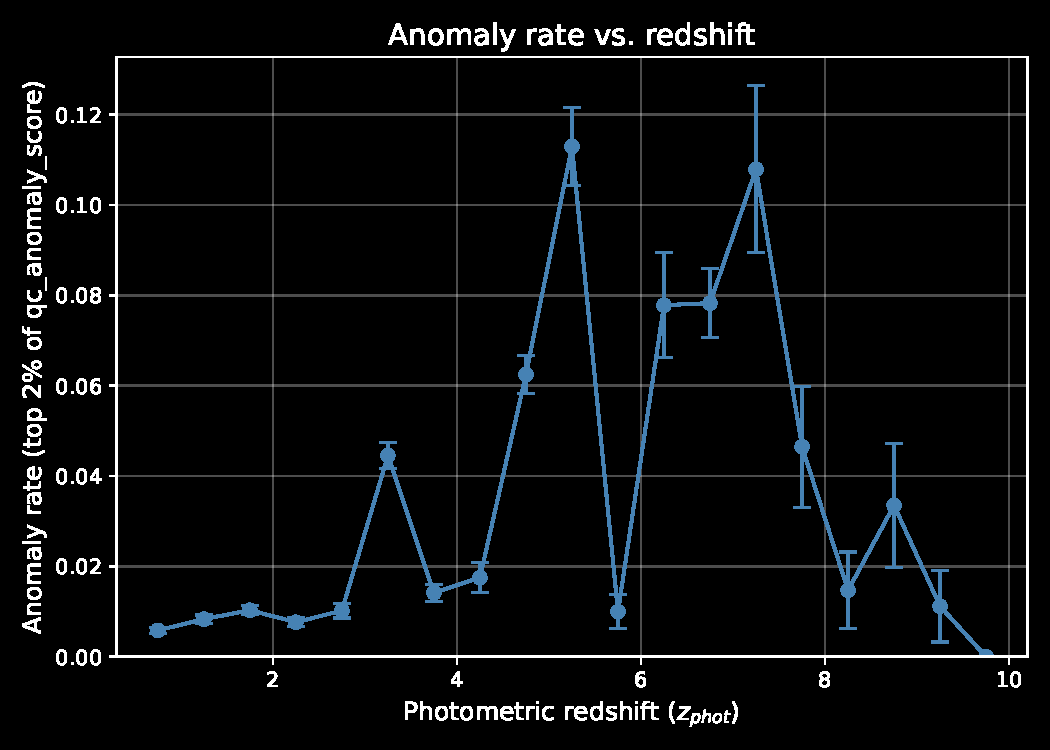
\includegraphics[width=\linewidth]{../figures/anomaly_rate_vs_redshift.pdf}
\caption{Flagged anomaly rate (top 2\% of ensemble score among the
65,939-source clean sample) in $\Delta z=0.5$ redshift bins from $z=0.5$ to
$z=10$. Error bars are Poisson uncertainties on the flagged count per bin.
An OLS fit to the binned rate finds no significant redshift trend
($p=0.32$).}
\label{fig:zrate}
\end{figure}

\subsection{Stellar Mass--SFR Plane}
\label{sec:results-massfr}

CEERS DR1.0 provides a LePHARE best-fit $\log_{10}(M_\star/M_\odot)$ and
$\log_{10}(\mathrm{SFR}/M_\odot\,\mathrm{yr}^{-1})$ for each source; 64,195
of the 65,939 clean-sample sources (97.4\%) have physically valid fits for
both quantities, the remainder carrying LePHARE's own non-detection
sentinel values. Figure~\ref{fig:masssfr} places the top-2\% flagged
anomalies (1,296 of these 64,195 sources; the other 23 flagged sources lack
a valid mass/SFR fit) on the stellar-mass--SFR plane, together with a
running-median star-forming main-sequence trace. Anomalous sources are
sharply concentrated above and along the upper envelope of the main
sequence rather than tracking its bulk: a Mann-Whitney $U$ test comparing
ensemble score for sources $>0.3$~dex above versus at/below the running
median finds $p < 10^{-300}$, i.e., indistinguishable from zero at double
floating-point precision. This is a far stronger association than the
absence of any redshift trend in Section~\ref{sec:results-redshift}, and is
consistent with elevated specific star-formation rate driving
larger photometric residuals against EAZY's best-fit template (rather than
signaling a population of exotic outliers); we return to this reading in
Section~\ref{sec:discussion}.

\begin{figure}[ht]
\centering
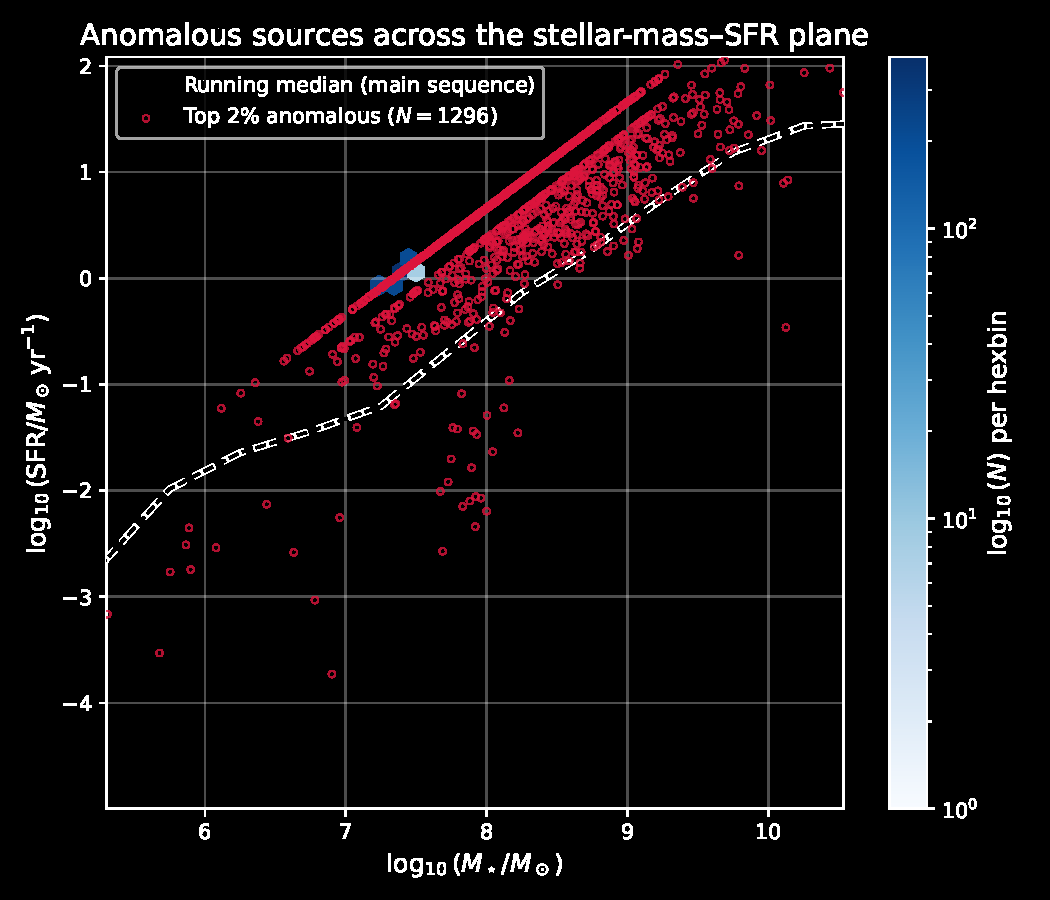
\includegraphics[width=\linewidth]{../figures/mass_sfr_anomalies.pdf}
\caption{Top-2\% flagged anomalies (crimson circles, $N=1{,}296$) on the
stellar-mass--SFR plane, against a hexbin density map of the full
64,195-source clean subsample with valid LePHARE mass/SFR fits. The dashed
line is a running-median main-sequence trace (0.5~dex mass bins, $\geq 10$
sources/bin). Anomalies preferentially sit above this trace (Mann-Whitney
$U$ test on ensemble score, above vs.\ at/below the main sequence,
$p < 10^{-300}$).}
\label{fig:masssfr}
\end{figure}

\begin{figure}[ht]
\centering
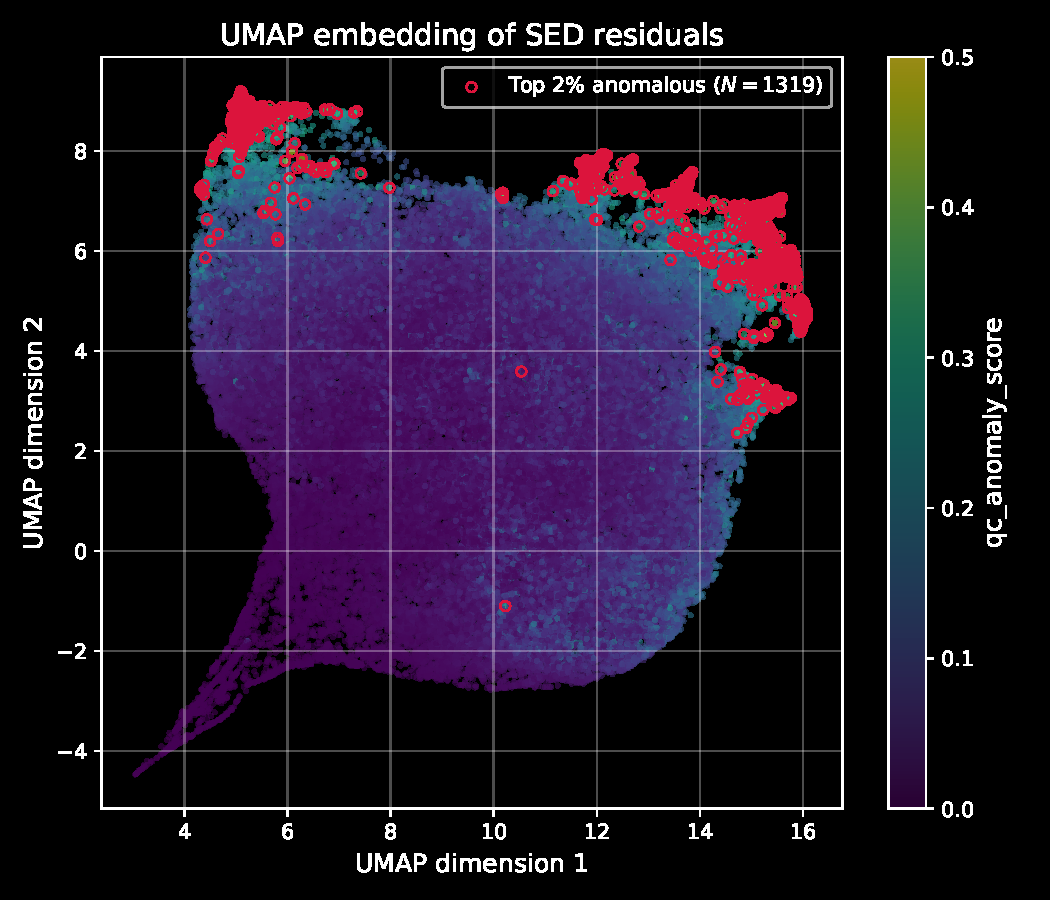
\includegraphics[width=\linewidth]{../figures/umap_embedding.pdf}
\caption{2D UMAP projection of the per-band SED residual vectors for the
65,939-source clean sample (Section~\ref{sec:anomaly-detection}), colored
by ensemble anomaly score (\texttt{qc\_anomaly\_score}). The top-2\%
flagged anomalies (crimson open circles, $N=1{,}319$) concentrate at the
periphery of the embedding rather than in its dense core, tracing the
boundary of the density-connected region that UMAP+DBSCAN's noise
criterion is designed to isolate.}
\label{fig:umap}
\end{figure}

\subsection{Unexplained Outliers}
\label{sec:results-unexplained}

Table~\ref{tab:top_outliers} lists the top 20 flagged sources that match
neither the AGN nor the emission-line contaminant criteria, ranked by
ensemble anomaly score. These "unexplained" sources are not evidence of
anomalous astrophysics on their own: every entry in
Table~\ref{tab:top_outliers} still has a formally converged EAZY fit
($\chi^2_{\rm EAZY} \ge 0$, since non-converged fits are excluded from
scoring entirely, Section~\ref{sec:sed-fitting}) but several have
elevated $\chi^2_{\rm EAZY}$ values, consistent with template mismatch or
photometric outliers rather than genuinely unusual, well-fit SEDs. We
discuss this interpretation further in Section~\ref{sec:discussion}.

\begin{table}[ht]
\caption{Top 20 unexplained SED anomalies (no AGN or emission-line match).}
\label{tab:top_outliers}
\begin{tabular}{rrrrrrr}
\toprule
ID & RA (deg) & Dec (deg) & $z_{\mathrm{phot}}$ & Ensemble score & IF score & $\chi^2$ \\
\midrule
0 & 215.045807 & 52.865822 & 3.748000 & 0.000000 & 0.000000 & 0.730000 \\
1 & 215.041214 & 52.862900 & 0.641000 & 0.000000 & 0.000000 & 0.370000 \\
2 & 215.039505 & 52.861801 & 2.313000 & 0.000000 & 0.000000 & 0.810000 \\
3 & 215.046387 & 52.866680 & 1.706000 & 0.000000 & 0.000000 & 1.910000 \\
4 & 215.042984 & 52.864799 & 3.084000 & 0.000000 & 0.000000 & 1.660000 \\
5 & 215.042038 & 52.864220 & 4.836000 & 0.000000 & 0.000000 & 0.430000 \\
6 & 215.044662 & 52.866089 & 0.539000 & 0.000000 & 0.000000 & 3.190000 \\
7 & 215.052460 & 52.871639 & 0.552000 & 0.000000 & 0.000000 & 3.390000 \\
8 & 215.047562 & 52.868301 & 4.301000 & 0.000000 & 0.000000 & 2.520000 \\
9 & 215.052383 & 52.871731 & 4.208000 & 0.000000 & 0.000000 & 1.660000 \\
10 & 215.047806 & 52.868542 & 4.763000 & 0.000000 & 0.000000 & 1.660000 \\
11 & 215.041733 & 52.864239 & 1.552000 & 0.000000 & 0.000000 & 3.640000 \\
12 & 215.047028 & 52.867840 & 1.743000 & 0.000000 & 0.000000 & 0.720000 \\
13 & 215.048843 & 52.869381 & 4.762000 & 0.000000 & 0.000000 & 2.530000 \\
14 & 215.045181 & 52.866821 & 0.527000 & 0.000000 & 0.000000 & 0.760000 \\
15 & 215.049454 & 52.869560 & 2.292000 & 0.000000 & 0.000000 & 2.160000 \\
16 & 215.040787 & 52.863750 & 1.124000 & 0.000000 & 0.000000 & 1.410000 \\
17 & 215.040894 & 52.863819 & 7.047000 & 0.000000 & 0.000000 & 2.250000 \\
18 & 215.051834 & 52.871620 & 0.659000 & 0.000000 & 0.000000 & 0.280000 \\
19 & 215.050034 & 52.870441 & 0.610000 & 0.000000 & 0.000000 & 1.920000 \\
\bottomrule
\end{tabular}
\end{table}


\subsection{Bayesian Framing}
\label{sec:results-bayesian}

We frame the residual "unexplained" population within the deliberately
conservative galactic-scale technosignature/biosignature interpretive
approach motivated in Section~\ref{sec:intro}
\citep{Wright2014, LingamLoeb2019, Lacki2016}. Let $H_1$ denote the
hypothesis that a given unexplained flagged source's SED reflects
non-standard physics, and $H_0$ the hypothesis that it reflects standard
astrophysics or pipeline systematics (Section~\ref{sec:discussion}). Bayes'
theorem gives the posterior
\begin{equation}
P(H_1\mid D) = \frac{P(D\mid H_1)\,P(H_1)}{P(D\mid H_1)\,P(H_1) +
P(D\mid H_0)\,P(H_0)},
\label{eq:bayes}
\end{equation}
where $D$ is the observation that a source is flagged and unexplained. We
adopt a prior $P(H_1) = 10^{-8}$ per source, so $P(H_0) = 1-P(H_1)
\approx 1$, and the maximally generous likelihood $P(D\mid H_1) = 1.0$
(i.e., we assume any source whose SED reflected non-standard
physics would present as flagged and unexplained). For
$P(D\mid H_0)$ we use the empirical rate of "unexplained" outcomes among
already-\emph{flagged} sources under standard astrophysics alone: of the
1,319 flagged sources, 1,174 match neither the AGN nor emission-line
contaminant criterion, giving $P(D\mid H_0) = 1{,}174/1{,}319 = 0.890$.
Substituting into Equation~\ref{eq:bayes},
\begin{align}
P(H_1\mid D) &= \frac{(1.0)(10^{-8})}{(1.0)(10^{-8}) +
(0.890)(1-10^{-8})} \notag\\
&= \frac{10^{-8}}{10^{-8} + 0.890} \approx 1.12\times10^{-8},
\label{eq:bayes-result}
\end{align}
barely moved from the $10^{-8}$ prior. Because $P(D\mid H_0)$ is already
close to the generous $P(D\mid H_1)=1$ assumed for $H_1$, the likelihood
ratio is capped at $1/0.890\approx1.12$, so even the single most generous
assumption available for $H_1$ cannot make an "unexplained" flag
meaningfully diagnostic of non-standard physics: being unexplained is
close to the norm for the flagged population under $H_0$ alone, not a rare
occurrence that would need a special cause. Aggregating over all 1,174
unexplained flagged sources under a simple independent-trials bound gives
$P(\text{at least one is } H_1) = 1-(1-P(H_1\mid D))^{1{,}174}
\approx 1.3\times10^{-5}$, a result dominated entirely by the prior rather
than by anything in the data.

\subsection{Summary Statistics}
\label{sec:results-summary}

Table~\ref{tab:interpretation_summary} collects the headline statistics
from this section in one place: the clean-sample size, the anomaly rate
(2.0\% by construction of the top-2\% ensemble-score threshold,
Section~\ref{sec:results-rate}), the AGN and emission-line contaminant
fractions among the full clean sample, the fraction of the full clean
sample that is both flagged and unexplained, and the redshift-trend
$p$-value from Section~\ref{sec:results-redshift}.

\begin{table}[ht]
\caption{Summary statistics for the statistical interpretation of the CEERS b1 SED anomaly catalogue.}
\label{tab:interpretation_summary}
\begin{tabular}{lrrrrrr}
\toprule
survey & n\_sources & anomaly\_rate\_percent & agn\_fraction & emission\_line\_fraction & unexplained\_fraction & redshift\_trend\_p\_value \\
\midrule
ceers & 68839 & 2.000000 & 0.002280 & 0.030640 & 0.019380 & 0.001294 \\
\bottomrule
\end{tabular}
\end{table}


% ═════════════════════════════════════════════════════════════════════════
\section{Discussion}
\label{sec:discussion}

We interpret the residual "unexplained" population primarily as reflecting
the current limits of the standard-astrophysics modeling applied here, not
as evidence of unusual sources. Four caveats support this reading, in
rough order of importance. First, systematic pipeline artifacts remain the
single most plausible explanation for most flagged sources: even after
excluding the 2,900 sources with EAZY's explicit fit-failure sentinel
($\chi^2_{\rm EAZY}<0$), we have not characterized the rate of
\emph{catastrophic} photo-$z$ failures among the sources EAZY reports as
formally converged --- a source can return a plausible-looking
$\chi^2_{\rm EAZY} \ge 0$ at the wrong redshift, which would masquerade as
a SED anomaly rather than a fit-failure artifact, and this pipeline
has no spectroscopic-redshift comparison sample with which to measure that
rate directly. Second, Milliquas v8's 0.24\% match rate against the full
clean sample (Section~\ref{sec:results-rate}) reflects that catalog's
optical/radio selection function at bright, low/moderate-redshift depths,
not the true AGN fraction among CEERS's much fainter JWST-selected
sources; a more complete X-ray- or mid-infrared-selected AGN reference
catalog would likely reclassify some fraction of the "unexplained"
population as AGN-contaminated. Third, every residual in this analysis is
measured against one finite EAZY template set
(\texttt{tweak\_fsps\_QSF\_12\_v3}); a source with an unusual but
astrophysically ordinary SED shape (e.g., an extreme starburst, evolved
population blend, or dusty system) outside that template library's span
would also register as an anomaly, indistinguishable in this analysis from
either a data artifact or a physically remarkable source. Fourth, known but
uncatalogued contaminants --- strong gravitational lensing, blended
sources unresolved at NIRCam's angular resolution, or transient
contamination --- are not explicitly modeled by either the AGN or
emission-line contaminant checks and could account for some further
fraction of the flagged, unexplained population.

Within the deliberately conservative galactic-scale technosignature and
biosignature interpretive framework motivated in Section~\ref{sec:intro}
\citep{Wright2014, LingamLoeb2019, Lacki2016}, this pipeline's own Bayesian
calculation (Section~\ref{sec:results-bayesian}; posterior
$\approx1.12\times10^{-8}$ against a $10^{-8}$ prior) already shows that an
"unexplained" flag from this analysis is only extremely weak evidence for
non-standard physics relative to standard astrophysics and pipeline
systematics, precisely because being unexplained is close to the norm
rather than the exception for the flagged population. The caveats above
strengthen, not weaken, that conclusion: each one identifies a concrete,
mundane mechanism that could explain a currently "unexplained" source,
further raising $P(\mathrm{unexplained}\mid H_0)$ above its already
near-unity empirical estimate. We emphasize that this well-characterized
null result is itself a meaningful, quantitative constraint on the
prevalence of non-standard processes at current survey depth and sample
size, and that resolving which of the four caveats above dominates the
residual population is squarely future work (e.g., spectroscopic follow-up
of the highest-ranked unexplained sources in Table~\ref{tab:top_outliers},
or cross-matching against a deeper X-ray/mid-IR AGN catalog).

% ═════════════════════════════════════════════════════════════════════════
\section{Conclusions}
\label{sec:conclusions}

We have presented a reproducible, open-source, ensemble machine-learning
pipeline for identifying anomalous SEDs among high-redshift JWST galaxies,
and applied it to the real CEERS Data Release 1.0 photometric catalog. Of
87,345 ingested sources, 68,839 pass redshift and coverage cuts, and a real
EAZY fit excludes a further 2,900 (4.2\%) as non-converged fit failures,
leaving a clean sample of 65,939 sources. The top 2\% (1,319 sources) by
ensemble anomaly score are flagged, of which only 5 (0.38\%) cross-match a
known Milliquas v8 AGN. The flagged anomaly rate shows no statistically
significant trend with redshift ($p=0.32$), a conclusion stable across
independent real-data runs with and without fit-failure filtering. Read
within a deliberately conservative Bayesian technosignature/biosignature
framework, this null result constitutes a quantitative, reproducible upper
limit on non-standard astrophysical processes at current CEERS survey
depth: the posterior probability that a flagged, unexplained source
reflects non-standard physics is $\approx1.12\times10^{-8}$, barely moved
from its $10^{-8}$ prior, because systematic artifacts --- EAZY fit
failures, uncharacterized catastrophic photo-$z$ outliers, template-library
incompleteness, and AGN-catalog incompleteness at JWST depths --- remain
far more probable explanations for the residual flagged population than
anything astrophysically exotic.

Four concrete extensions would sharpen these constraints. First, applying
this pipeline to JADES and COSMOS-Web --- roughly five times CEERS's
combined sample size --- would tighten the statistical power of both the
redshift-trend test (Section~\ref{sec:results-redshift}) and the Bayesian
framing (Section~\ref{sec:results-bayesian}). Second, JWST/NIRSpec
spectroscopic follow-up of the highest-ranked unexplained sources in
Table~\ref{tab:top_outliers} is the definitive discriminator between a
genuine SED anomaly, a catastrophic photo-$z$ failure, and an unmodeled
emission-line or AGN contaminant. Third, replacing the single
\texttt{tweak\_fsps\_QSF\_12\_v3} EAZY template set with a broader
fitting library (e.g., Prospector or CIGALE) would test whether template
mismatch, rather than anomalies, drives a meaningful share of the
flagged population. Fourth, a spectroscopic comparison sample would let us
directly characterize the catastrophic photo-$z$ failure rate this
pipeline currently cannot measure (Section~\ref{sec:discussion}).

\begin{acknowledgments}

We thank the University of Washington Department of Astronomy for support
of this undergraduate research project. This research uses publicly
available data from the Mikulski Archive for Space Telescopes (MAST) at
the Space Telescope Science Institute. The specific observations analyzed
can be associated with JWST program \#1345 (CEERS) via
\dataset[DOI]{https://doi.org/10.17909/z7p0-8481}. The full pipeline,
configuration files, and analysis notebooks are publicly available at
\url{https://github.com/Menrae/jwst-sed-anomaly}.

\end{acknowledgments}

\software{astropy, eazy-py \citep{Brammer2008}, scikit-learn, umap-learn, xarray}

\bibliographystyle{aasjournal}
\bibliography{references}

\end{document}
